\chapter{Verkkojen perusteet}

Voimme ratkaista monia algoritmisia ongelmia
esittämällä tilanteen \emph{verkkona} ja käyttämällä sitten
sopivaa verkkoalgoritmia.
Tyypillinen esimerkki verkosta on tieverkosto,
joka muodostuu kaupungeista ja niiden välisistä teistä.
Tällaisessa verkossa ongelmana voi olla selvittää vaikkapa,
kuinka voimme matkustaa kaupungista $a$ kaupunkiin $b$.

Tässä luvussa aloitamme verkkoihin tutustumisen
käymällä läpi verkkojen käsitteitä sekä tapoja
esittää verkkoja ohjelmoinnissa.
Tämän jälkeen näemme, miten voimme tutkia verkkojen rakennetta
ja ominaisuuksia syvyyshaun ja leveyshaun avulla.
Seuraavissa kirjan luvuissa jatkamme verkkojen käsittelyä ja
opimme lisää verkkoalgoritmeja.

\section{Verkkojen käsitteitä}

Verkko muodostuu \emph{solmuista} ja
niitä yhdistävistä \emph{kaarista}.
Esimerkiksi kuvassa \ref{fig:veresi} on verkko,
jossa on viisi solmua ja seitsemän kaarta.
Merkitsemme verkon solmujen
määrää kirjaimella $n$ ja kaarten määrää
kirjaimella $m$.
Lisäksi numeroimme verkon solmut kokonaisluvuin
$1,2,\dots,n$.

\begin{figure}
\center
\begin{center}
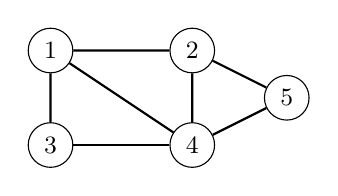
\begin{tikzpicture}[scale=0.6]
\small
\node[draw, circle] (1) at (1,3) {$1$};
\node[draw, circle] (2) at (4,3) {$2$};
\node[draw, circle] (3) at (1,1) {$3$};
\node[draw, circle] (4) at (4,1) {$4$};
\node[draw, circle] (5) at (6,2) {$5$};

\path[draw,thick,-] (1) -- (2);
\path[draw,thick,-] (1) -- (3);
\path[draw,thick,-] (1) -- (4);
\path[draw,thick,-] (3) -- (4);
\path[draw,thick,-] (2) -- (4);
\path[draw,thick,-] (2) -- (5);
\path[draw,thick,-] (4) -- (5);
\end{tikzpicture}
\end{center}
\caption{Verkko, jossa on viisi solmua ja seitsemän kaarta.}
\label{fig:veresi}
\end{figure}

Sanomme, että kaksi solmua ovat \emph{vierekkäin} verkossa,
jos niiden välillä on kaari.
Solmun \emph{naapureja} ovat kaikki solmut,
joihin se on yhteydessä kaarella,
ja solmun \emph{aste} on sen naapureiden määrä.
Kuvassa \ref{fig:veresi} solmun 2 naapurit ovat 1, 4 ja 5,
joten solmun aste on 3.
Voimme kulkea solmusta 1 solmuun 5
esimerkiksi polkua $1 \rightarrow 2 \rightarrow 5$
tai $1 \rightarrow 3 \rightarrow 4 \rightarrow 5$.

\subsubsection{Polku ja sykli}

Verkossa oleva \emph{polku} solmusta $a$ solmuun $b$
on reitti solmusta $a$ solmuun $b$ kaaria pitkin.
Kuvassa \ref{fig:veresi}
voimme kulkea solmusta $1$ solmuun $5$
vaikkapa polkua $1 \rightarrow 2 \rightarrow 5$
tai polkua
$1 \rightarrow 3 \rightarrow 4 \rightarrow 5$.

Polku on \emph{sykli},
jos se alkaa ja päättyy samassa solmussa,
kulkee ainakin yhden toisen solmun kautta
eikä kulje kahta kertaa saman solmun tai kaaren kautta.
Kuvassa \ref{fig:veresi} on esimerkiksi sykli
$2 \rightarrow 4 \rightarrow 5 \rightarrow 2$.
Jos verkossa ei ole yhtään sykliä, verkko on \emph{syklitön}.

\subsubsection{Yhtenäisyys ja komponentit}

Verkko on \emph{yhtenäinen},
jos minkä tahansa kahden solmun välillä on polku.
Kuvan \ref{fig:veresi} verkko on yhtenäinen,
mutta kuvan \ref{fig:veryht} verkko ei ole yhtenäinen,
koska esimerkiksi solmujen $1$ ja $2$ välillä ei ole polkua.

Voimme esittää verkon aina kokoelmana yhtenäisiä \emph{komponentteja}.
Kuvassa \ref{fig:veryht} yhtenäiset komponentit
ovat $\{1,3\}$ ja $\{2,4,5\}$.

\begin{figure}
\center
\begin{center}
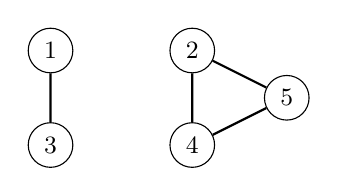
\begin{tikzpicture}[scale=0.6]
\small
\node[draw, circle] (1) at (1,3) {$1$};
\node[draw, circle] (2) at (4,3) {$2$};
\node[draw, circle] (3) at (1,1) {$3$};
\node[draw, circle] (4) at (4,1) {$4$};
\node[draw, circle] (5) at (6,2) {$5$};

\path[draw,thick,-] (1) -- (3);
\path[draw,thick,-] (2) -- (4);
\path[draw,thick,-] (2) -- (5);
\path[draw,thick,-] (4) -- (5);
\end{tikzpicture}
\end{center}
\caption{Verkon yhtenäiset komponentit ovat $\{1,3\}$ ja $\{2,4,5\}$.}
\label{fig:veryht}
\end{figure}

\subsubsection{Puu}

Verkko on \emph{puu}, jos se on sekä yhtenäinen
että syklitön.
Puussa kaarten määrä on aina yhden pienempi
kuin solmujen määrä, ja jokaisen kahden solmun
välillä on yksikäsitteinen polku.
Kuvassa \ref{fig:verpuu} on esimerkkinä puu,
jossa on viisi solmua ja neljä kaarta.

\begin{figure}
\center
\begin{center}
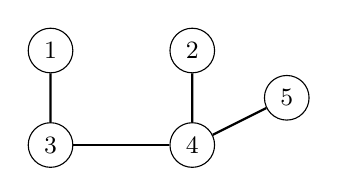
\begin{tikzpicture}[scale=0.6]
\small
\node[draw, circle] (1) at (1,3) {$1$};
\node[draw, circle] (2) at (4,3) {$2$};
\node[draw, circle] (3) at (1,1) {$3$};
\node[draw, circle] (4) at (4,1) {$4$};
\node[draw, circle] (5) at (6,2) {$5$};

\path[draw,thick,-] (1) -- (3);
\path[draw,thick,-] (3) -- (4);
\path[draw,thick,-] (2) -- (4);
\path[draw,thick,-] (4) -- (5);
\end{tikzpicture}
\end{center}
\caption{Yhtenäinen, syklitön verkko eli puu.}
\label{fig:verpuu}
\end{figure}

\subsubsection{Suunnattu verkko}

Kun verkko on \emph{suunnattu},
jokaisella kaarella on tietty suunta,
jonka mukaisesti meidän täytyy kulkea kaarta pitkin.
Suunnat rajoittavat siis liikkumistamme verkossa.

Kuvassa \ref{fig:versuu} on esimerkkinä
suunnattu verkko.
Tässä verkossa voimme kulkea solmusta $1$ solmuun $5$
polkua $1 \rightarrow 2 \rightarrow 5$,
mutta verkossa ei ole mitään polkua solmusta $5$ solmuun $1$.

\begin{figure}
\center
\begin{center}
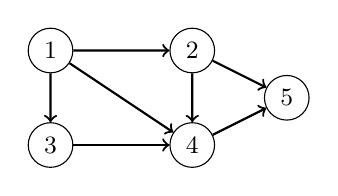
\begin{tikzpicture}[scale=0.6]
\small
\node[draw, circle] (1) at (1,3) {$1$};
\node[draw, circle] (2) at (4,3) {$2$};
\node[draw, circle] (3) at (1,1) {$3$};
\node[draw, circle] (4) at (4,1) {$4$};
\node[draw, circle] (5) at (6,2) {$5$};

\path[draw,thick,->] (1) -- (2);
\path[draw,thick,->] (1) -- (3);
\path[draw,thick,->] (1) -- (4);
\path[draw,thick,->] (3) -- (4);
\path[draw,thick,->] (2) -- (4);
\path[draw,thick,->] (2) -- (5);
\path[draw,thick,->] (4) -- (5);
\end{tikzpicture}
\end{center}
\caption{Suunnattu verkko.}
\label{fig:versuu}
\end{figure}

\subsubsection{Painotettu verkko}

Kun verkko on \emph{painotettu},
jokaiseen kaareen liittyy jokin paino,
joka kuvaa usein kaaren pituutta.
Kun kuljemme polkua painotetussa verkossa,
polun pituus on kaarten painojen summa.

Kuvassa \ref{fig:verpai} on esimerkkinä painotettu verkko.
Tässä verkossa polun $1 \rightarrow 2 \rightarrow 5$
paino on $5+8=13$ ja polun
$1 \rightarrow 3 \rightarrow 4 \rightarrow 5$
paino on $2+4+3=9$.

\begin{figure}
\center
\begin{center}
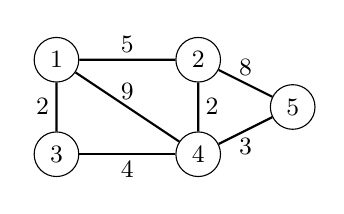
\begin{tikzpicture}[scale=0.6,label distance=-1.5mm]
\small
\node[draw, circle] (1) at (1,3) {$1$};
\node[draw, circle] (2) at (4,3) {$2$};
\node[draw, circle] (3) at (1,1) {$3$};
\node[draw, circle] (4) at (4,1) {$4$};
\node[draw, circle] (5) at (6,2) {$5$};

\path[draw,thick,-] (1) -- node[font=\small,label=above:5] {} (2);
\path[draw,thick,-] (1) -- node[font=\small,label=left:2] {} (3);
\path[draw,thick,-] (1) -- node[font=\small,label=above:9] {} (4);
\path[draw,thick,-] (3) -- node[font=\small,label=below:4] {} (4);
\path[draw,thick,-] (2) -- node[font=\small,label=above:8] {} (5);
\path[draw,thick,-] (4) -- node[font=\small,label=right:2] {} (2);
\path[draw,thick,-] (4) -- node[font=\small,label=below:3] {} (5);
\end{tikzpicture}
\end{center}
\caption{Painotettu verkko.}
\label{fig:verpai}
\end{figure}


\section{Verkot ohjelmoinnissa}

Verkon esittämiseen ohjelmoinnissa on monia mahdollisuuksia.
Sopivan esitystavan valintaan vaikuttaa,
miten haluamme käsitellä verkkoa algoritmissa,
koska jokaisessa esitystavassa on omat etunsa.
Seuraavaksi käymme läpi kolme tavallista esitystapaa.

\subsection{Vieruslistaesitys}

Vieruslistaesityksessä luomme kullekin verkon solmulle
\emph{vieruslistan}, joka kertoo, mihin solmuihin voimme
siirtyä solmusta kaaria pitkin.
Esimerkiksi Javassa voimme luoda taulukon

\begin{code}
ArrayList<Integer>[] verkko = new ArrayList<>[n+1];
\end{code}

ja alustaa vieruslistat näin:

\begin{code}
for (int i = 1; i <= n; i++) {
    verkko[i] = new ArrayList<>();
}
\end{code}

Voimme luoda esimerkiksi kuvan \ref{fig:versuu}
verkon seuraavasti:

\begin{code}
verkko[1].add(2);
verkko[1].add(3);
verkko[1].add(4);
verkko[2].add(4);
verkko[2].add(5);
verkko[3].add(4);
verkko[4].add(5);
\end{code}

Vieruslistaesitys on usein hyvä tapa tallentaa verkko,
koska monessa algoritmissa haluamme selvittää,
mihin solmuihin pääsemme siirtymään tietystä solmusta kaaria pitkin.

\subsection{Kaarilistaesitys}

Kaarilistaesityksessä luomme listan,
jossa on kaikki verkon kaaret:

\begin{code}
ArrayList<Kaari> kaaret = new ArrayList<>();
\end{code}

Voimme tallentaa kaaret esimerkiksi seuraavasti:

\begin{code}
public class Kaari {
    public int alku, loppu;

    public Kaari(int alku, int loppu) {
        this.alku = alku;
        this.loppu = loppu;
    }
}
\end{code}

Seuraava koodi luo kuvan \ref{fig:versuu}
verkkoa vastaavan kaarilistan:

\begin{code}
kaaret.add(new Kaari(1,2));
kaaret.add(new Kaari(1,3));
kaaret.add(new Kaari(1,4));
kaaret.add(new Kaari(2,4));
kaaret.add(new Kaari(2,5));
kaaret.add(new Kaari(3,4));
kaaret.add(new Kaari(4,5));
\end{code}

Kaarilista on hyvä esitystapa algoritmeissa,
joissa meidän täytyy pystyä käymään helposti läpi
kaikki verkon kaaret.

\subsection{Vierusmatriisiesitys}

Vierusmatriisi on kaksiulotteinen taulukko,
joka kertoo jokaisesta verkon kaaresta,
esiintyykö se verkossa.
Jos verkossa on kaari $a \rightarrow b$,
niin matriisin rivin $a$ sarakkeessa $b$
on sitä vastaava merkintä.
Voimme määritellä matriisin seuraavasti:

\begin{code}
int[][] verkko = new int[n+1][n+1];
\end{code}

Seuraava koodi rakentaa matriisin,
joka vastaa kuvan \ref{fig:versuu} verkkoa.
Tässä matriisin jokainen alkio on 0 (ei kaarta)
tai 1 (kaari).

\begin{code}
verkko[1][2] = 1;
verkko[1][3] = 1;
verkko[1][4] = 1;
verkko[2][4] = 1;
verkko[2][5] = 1;
verkko[3][4] = 1;
verkko[4][5] = 1;
\end{code}

Vierusmatriisin etuna on, että voimme tarkastaa helposti,
onko tietty kaari verkossa.
Esitystapa kuluttaa kuitenkin paljon muistia,
eikä sitä voi käyttää, jos verkon solmujen määrä on suuri.

\section{Syvyyshaku}

\emph{Syvyyshaku} on verkkojen käsittelyn perusalgoritmi,
joka etsii kaikki solmut, jotka ovat saavutettavissa
annetusta lähtösolmusta.
Voimme selvittää syvyyshaun avulla monia asioita
verkon rakenteesta.

Syvyyshaku lähtee liikkeelle tietystä verkon solmusta
ja alkaa tutkia verkkoa siitä käsin.
Algoritmi pitää yllä jokaisesta solmusta tietoa,
onko se vielä vieraillut solmussa.
Kun haku saapuu solmuun, jossa se ei ole käynyt aiemmin,
se merkitsee solmun vierailluksi ja
etenee syvemmälle verkossa jatkamalla hakua
yksi kerrallaan solmusta lähteviä kaaria pitkin.
Tämän jälkeen algoritmi perääntyy taaksepäin
samaa polkua kuin tuli solmuun.

\begin{figure}
\center
\begin{center}
\begin{tikzpicture}[scale=0.6]
\scriptsize
\newcommand\verkko[6]{
\node[draw, circle, fill=#2] (1) at (0,0) {$1$};
\node[draw, circle, fill=#3] (2) at (2,0) {$2$};
\node[draw, circle, fill=#4] (3) at (0,-2) {$3$};
\node[draw, circle, fill=#5] (4) at (2,-2) {$4$};
\node[draw, circle, fill=#6] (5) at (4,-1) {$5$};
\path[draw,thick,-] (1) -- (2);
\path[draw,thick,-] (2) -- (5);
\path[draw,thick,-] (2) -- (4);
\path[draw,thick,-] (4) -- (5);
\path[draw,thick,-] (1) -- (3);
\node at (2,-3) {vaihe #1};
}
\begin{scope}
\verkko{1}{lightgray}{white}{white}{white}{white}
\end{scope}
\begin{scope}[xshift=6cm]
\verkko{2}{lightgray}{lightgray}{white}{white}{white}
\path[draw=red,thick,->,line width=2pt] (1) -- (2);
\end{scope}
\begin{scope}[xshift=12cm]
\verkko{3}{lightgray}{lightgray}{white}{lightgray}{white}
\path[draw=red,thick,->,line width=2pt] (1) -- (2);
\path[draw=red,thick,->,line width=2pt] (2) -- (4);
\end{scope}
\begin{scope}[xshift=18cm]
\verkko{4}{lightgray}{lightgray}{white}{lightgray}{lightgray}
\path[draw=red,thick,->,line width=2pt] (1) -- (2);
\path[draw=red,thick,->,line width=2pt] (2) -- (4);
\path[draw=red,thick,->,line width=2pt] (4) -- (5);
\end{scope}
\begin{scope}[yshift=-5cm]
\verkko{5}{lightgray}{lightgray}{white}{lightgray}{lightgray}
\path[draw=red,thick,->,line width=2pt] (1) -- (2);
\path[draw=red,thick,->,line width=2pt] (2) -- (4);
\path[draw=red,thick,->,line width=2pt] (4) -- (5);
\path[draw=red,thick,->,line width=2pt] (5) -- (2);
\end{scope}
\begin{scope}[yshift=-5cm,xshift=6cm]
\verkko{6}{lightgray}{lightgray}{white}{lightgray}{lightgray}
\path[draw=red,thick,->,line width=2pt] (1) -- (2);
\path[draw=red,thick,->,line width=2pt] (2) -- (4);
\path[draw=red,thick,->,line width=2pt] (4) -- (5);
\end{scope}
\begin{scope}[yshift=-5cm,xshift=12cm]
\verkko{7}{lightgray}{lightgray}{white}{lightgray}{lightgray}
\path[draw=red,thick,->,line width=2pt] (1) -- (2);
\path[draw=red,thick,->,line width=2pt] (2) -- (4);
\end{scope}
\begin{scope}[yshift=-5cm,xshift=18cm]
\verkko{8}{lightgray}{lightgray}{white}{lightgray}{lightgray}
\path[draw=red,thick,->,line width=2pt] (1) -- (2);
\end{scope}
\begin{scope}[yshift=-10cm]
\verkko{9}{lightgray}{lightgray}{white}{lightgray}{lightgray}
\end{scope}
\begin{scope}[yshift=-10cm,xshift=6cm]
\verkko{10}{lightgray}{lightgray}{lightgray}{lightgray}{lightgray}
\path[draw=red,thick,->,line width=2pt] (1) -- (3);
\end{scope}
\begin{scope}[yshift=-10cm,xshift=12cm]
\verkko{11}{lightgray}{lightgray}{lightgray}{lightgray}{lightgray}
\end{scope}
\end{tikzpicture}
\end{center}
\caption{Esimerkki syvyyshaun toiminnasta.}
\label{fig:syvhak}
\end{figure}

Kuvassa \ref{fig:syvhak} on esimerkki syvyyshaun toiminnasta.
Jokaisessa vaiheessa harmaat solmut ovat solmuja,
joissa haku on jo vieraillut.
Haku lähtee liikkeelle solmusta 1,
josta pääsee solmuihin 2 ja 3.
Haku etenee ensin solmuun 2, josta pääsee edelleen
solmuihin 4 ja 5.
Koska haku ei enää pysty etenemään solmusta 5,
se perääntyy takaisin solmuun 1.
Tämän jälkeen haku käy vielä solmussa 3,
minkä jälkeen se on käynyt läpi kaikki solmut,
joihin pääsee solmusta 1.

\subsection{Algoritmin toteutus}

Syvyyshaku on mukavaa toteuttaa rekursiivisesti.
Tarvitsemme ensinnäkin taulukon, joka kertoo,
missä solmuissa olemme käyneet:

\begin{code}
boolean[] vierailtu = new boolean[n+1];
\end{code}

Tämän jälkeen voimme toteuttaa syvyyshaun näin
käyttäen verkon vieruslistaesitystä:

\begin{code}
void syvyyshaku(int solmu) {
    if (vierailtu[solmu]) return;
    vierailtu[solmu] = true;
    for (Integer naapuri : verkko[solmu]) {
        syvyyshaku(naapuri);
    }
}
\end{code}

Syvyyshaku käynnistyy, kun kutsumme metodia
\texttt{syvyyshaku} parametrina lähtösolmu.
Jokaisella kutsulla metodi tarkistaa ensin,
olemmeko jo käyneet parametrina annetussa solmussa,
ja päättyy heti tässä tilanteessa.
Muuten metodi merkitsee, että olemme nyt käyneet solmussa
ja etenee rekursiivisesti kaikkiin solmun naapureihin.

Syvyyshaku käsittelee kerran jokaisen solmun,
johon pääsee lähtösolmusta,
käymällä läpi siitä lähtevät kaaret.
Niinpä syvyyshaku vie aikaa $O(n+m)$, missä $n$ on
verkon solmujen määrä ja $m$ on verkon kaarten määrä.

\subsection{Sovelluksia}

Syvyyshaku on yleistyökalu verkko-ongelmien ratkaisemiseen.
Seuraavassa on joitakin esimerkkejä syvyyshaun käyttökohteista.
Oletamme, että verkko on suuntaamaton, eli voimme kulkea
kaikkia kaaria kumpaankin suuntaan.

\subsubsection{Polun etsiminen}

Syvyyshaun avulla voimme etsiä verkosta polun solmusta
$a$ solmuun $b$, jos tällainen polku on olemassa.
Tämä tapahtuu aloittamalla haku solmusta $a$
ja pysähtymällä, kun vastaan tulee solmu $b$.
Jos polkuja on useita, syvyyshaku löytää jonkin niistä
riippuen solmujen käsittelyjärjestyksestä.

\subsubsection{Yhtenäisyys ja komponentit}

Verkko on yhtenäinen, jos kaikki solmut ovat yhteydessä
toisiinsa.
Voimmekin tarkastaa verkon yhtenäisyyden aloittamalla
syvyyshaun mielivaltaisesta solmusta ja tutkimalla,
saavuttaako haku kaikki verkon solmut.
Lisäksi voimme löytää verkon yhtenäiset komponentit
käymällä läpi solmut ja aloittamalla syvyyshaun aina,
kun vastaan tulee uusi solmu.
Jokainen syvyyshaku muodostaa yhden komponentin.

\subsubsection{Syklin etsiminen}

Jos verkossa on sykli, huomaamme sen syvyyshaun aikana siitä,
että tulemme tulemme toista kautta johonkin solmuun,
jossa olemme käyneet jo aiemmin.
Niinpä löydämme syvyyshaun avulla jonkin verkossa olevan
syklin, jos sellainen on olemassa.

\section{Leveyshaku}

\emph{Leveyshaku} on algoritmi, joka selvittää \emph{lyhimmän} polun
lähtösolmusta kaikkiin solmuihin, jotka ovat saavutettavissa siitä.
Lyhin polku tarkoittaa tässä polkua, jossa on mahdollisimman vähän kaaria.
Ideana on käsitellä solmut kerroksittain lähtösolmusta alkaen
siinä järjestyksessä kuin olemme löytäneet ne.
Jokaisen solmun kohdalla käymme läpi kaikki siitä lähtevät kaaret.

\begin{figure}
\center
\begin{center}
\begin{tikzpicture}[scale=0.6]
\scriptsize
\newcommand\verkko[6]{
\node[draw, circle, fill=#2] (1) at (0,0) {$1$};
\node[draw, circle, fill=#3] (2) at (2,0) {$2$};
\node[draw, circle, fill=#4] (3) at (0,-2) {$3$};
\node[draw, circle, fill=#5] (4) at (2,-2) {$4$};
\node[draw, circle, fill=#6] (5) at (4,-1) {$5$};
\path[draw,thick,-] (1) -- (2);
\path[draw,thick,-] (2) -- (5);
\path[draw,thick,-] (2) -- (4);
\path[draw,thick,-] (4) -- (5);
\path[draw,thick,-] (1) -- (3);
\node at (2,-3) {vaihe #1};
}
\begin{scope}
\verkko{1}{lightgray}{white}{white}{white}{white}
\end{scope}
\begin{scope}[xshift=6cm]
\verkko{2}{lightgray}{lightgray}{white}{white}{white}
\path[draw=red,thick,->,line width=2pt] (1) -- (2);
\end{scope}
\begin{scope}[xshift=12cm]
\verkko{3}{lightgray}{lightgray}{lightgray}{white}{white}
\path[draw=red,thick,->,line width=2pt] (1) -- (3);
\end{scope}
\begin{scope}[xshift=18cm]
\verkko{4}{lightgray}{lightgray}{lightgray}{white}{white}
\path[draw=red,thick,->,line width=2pt] (2) -- (1);
\end{scope}
\begin{scope}[yshift=-5cm,xshift=0cm]
\verkko{5}{lightgray}{lightgray}{lightgray}{lightgray}{white}
\path[draw=red,thick,->,line width=2pt] (2) -- (4);
\end{scope}
\begin{scope}[yshift=-5cm,xshift=6cm]
\verkko{6}{lightgray}{lightgray}{lightgray}{lightgray}{lightgray}
\path[draw=red,thick,->,line width=2pt] (2) -- (5);
\end{scope}
\begin{scope}[yshift=-5cm,xshift=12cm]
\verkko{7}{lightgray}{lightgray}{lightgray}{lightgray}{lightgray}
\path[draw=red,thick,->,line width=2pt] (3) -- (1);
\end{scope}
\begin{scope}[yshift=-5cm,xshift=18cm]
\verkko{8}{lightgray}{lightgray}{lightgray}{lightgray}{lightgray}
\path[draw=red,thick,->,line width=2pt] (4) -- (2);
\end{scope}
\begin{scope}[yshift=-10cm,xshift=0cm]
\verkko{9}{lightgray}{lightgray}{lightgray}{lightgray}{lightgray}
\path[draw=red,thick,->,line width=2pt] (4) -- (5);
\end{scope}
\begin{scope}[yshift=-10cm,xshift=6cm]
\verkko{10}{lightgray}{lightgray}{lightgray}{lightgray}{lightgray}
\path[draw=red,thick,->,line width=2pt] (5) -- (2);
\end{scope}
\begin{scope}[yshift=-10cm,xshift=12cm]
\verkko{11}{lightgray}{lightgray}{lightgray}{lightgray}{lightgray}
\path[draw=red,thick,->,line width=2pt] (5) -- (4);
\end{scope}
\end{tikzpicture}
\end{center}
\caption{Esimerkki leveyshaun toiminnasta.}
\label{fig:levhak}
\end{figure}

Kuvassa \ref{fig:levhak} on esimerkki leveyshaun toiminnasta,
kun etsimme polkuja solmusta 1 aloittaen.
Käsittelemme ensin solmun 1, josta pääsemme uusiin solmuihin 2 ja 3.
Tämä tarkoittaa, että lyhimmät polut solmuihin 2 ja 3
ovat $1 \rightarrow 2$ ja $1 \rightarrow 3$.
Sitten käsittelemme solmun 2, josta pääsemme uusiin solmuihin 4 ja 5.
Tämä tarkoittaa, että lyhimmät polut solmuihin 4 ja 5
ovat $1 \rightarrow 2 \rightarrow 4$ ja $1 \rightarrow 2 \rightarrow 5$.
Lopuksi käsittelemme vielä solmut 3, 4 ja 5,
joista emme kuitenkaan pääse enää uusiin solmuihin.

\subsection{Algoritmin toteutus}

Leveyshaku on vaikeampi toteuttaa kuin syvyyshaku,
koska meidän täytyy pystyä edistämään hakua vuorotellen verkon eri puolilta.
Tätä varten luomme \emph{jonon}, joka sisältää läpikäyntiä odottavia solmuja.
Valitsemme aina seuraavaksi käsiteltävän solmun jonon alusta,
ja lisämme uudet vieraillut solmut jonon loppuun.
Voimme luoda jonon näin:

\begin{code}
ArrayDeque<Integer> jono = new ArrayDeque<>();
\end{code}

Lisäksi määrittelemme syvyyshaun tapaan taulukon, jossa pidämme kirjaa,
missä solmuissa olemme käyneet:

\begin{code}
boolean[] vierailtu = new boolean[n+1];
\end{code}

Oletamme seuraavassa koodissa, että aloitamme leveyshaun solmusta \texttt{alku} alkaen.
Voimme toteuttaa haun seuraavasti:

\begin{code}
vierailtu[alku] = true;
jono.addLast(alku);
while (jono.size() > 0) {
    int solmu = jono.pollFirst();
    for (int naapuri : verkko[solmu]) {
        if (vierailtu[naapuri]) continue;
        vierailtu[naapuri] = true;
        jono.addLast(naapuri);
    }
}
\end{code}

Koodi merkitsee aluksi, että olemme käyneet lähtösolmussa
sekä lisää lähtösolmun jonoon.
Tämän jälkeen joka askeleella haku valitsee
jonon ensimmäisen solmun ja tarkastaa siitä lähtevät kaaret.
Jos pääsemme uuteen solmuun, merkitsemme uuden solmun
vierailluksi ja lisäämme sen jonoon.
Haku jatkuu niin kauan kuin jonossa on solmuja.

Syvyyshaun tavoin leveyshaku vie aikaa $O(n+m)$,
koska käymme läpi kerran jokaisesta solmusta lähtevät kaaret.

\subsection{Polkujen etsiminen}

Vaikka leveyshakua voi käyttää yleisalgoritmina verkon läpikäyntiin,
yleensä tavoitteena on nimenomaan löytää lyhimmät polut lähtösolmusta
muihin solmuihin. Tätä varten määrittelemme kaksi uutta taulukkoa:

\begin{code}
int[] etaisyys = new int[n+1];
int[] aiempi = new int[n+1];
\end{code}

Taulukko \texttt{etaisyys} kertoo, mikä on etäisyys
(eli lyhimmän polun pituus) lähtösolmusta kyseiseen solmuun,
ja taulukko \texttt{aiempi} viittaa edelliseen solmuun lyhimmällä polulla.
Näiden taulukoiden avulla voimme leveyshaun jälkeen muodostaa
lyhimmän polun lähtösolmusta mihin tahansa solmuun.
Päivitäm\-me taulukoita seuraavasti haun aikana:

\begin{code}
vierailtu[alku] = true;
etaisyys[alku] = 0;
aiempi[alku] = 0;
jono.addLast(alku);
while (jono.size() > 0) {
    int solmu = jono.pollFirst();
    for (int naapuri : verkko[solmu]) {
        if (vierailtu[naapuri]) continue;
        vierailtu[naapuri] = true;
        etaisyys[naapuri] = etaisyys[solmu]+1;
        aiempi[naapuri] = solmu;
        jono.addLast(naapuri);
    }
}
\end{code}

Haun alussa merkitsemme, että etäisyys lähtösolmuun on 0
ja sillä ei ole edellistä solmua.
Sitten kun löydämme uuden solmun, päivitämme sen etäisyyden
ja edellisen solmun polulla.

Nyt leveyshaun jälkeen lyhimmän polun pituus lähtösolmusta
solmuun $x$ on $\texttt{etaisyys}[x]$ ja voimme käydä läpi polulla
olevat solmut seuraavasti (käänteisessä järjestyksessä):

\begin{code}
while (x != 0) {
    System.out.println(x);
    x = aiempi[x];
}
\end{code}

\section{Esimerkki: Labyrintti}

Olemme labyrintissa ja haluamme päästä ruudusta $A$ ruutuun $B$.
Joka askeleella voimme siirtyä yhden ruudun verran ylöspäin, alaspäin,
vasemmalle tai oikealle.
Pystymmekö pääsemään ruudusta $A$ ruutuun $B$, ja jos pystymme, niin
mikä on lyhin mahdollinen reitti?
Esimerkiksi kuvassa \ref{fig:labrei}(a) lyhin reitti
ruudusta $A$ ruutuun $B$ muodostuu 9 askeleesta.

\begin{figure}
\center
\begin{center}
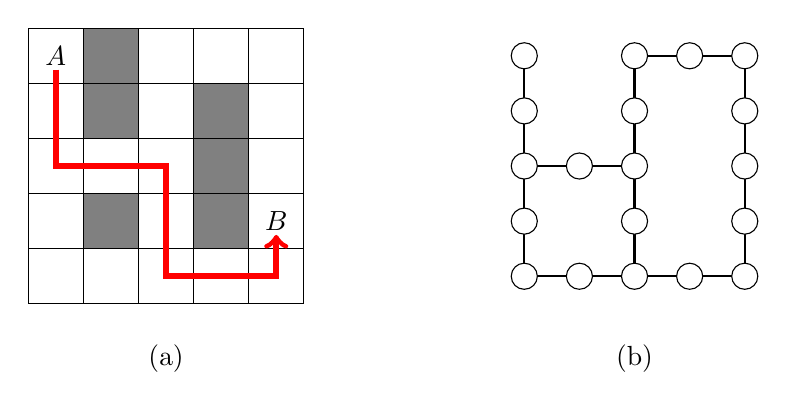
\begin{tikzpicture}[scale=0.7]
\begin{scope}
\draw[fill=gray] (1,1) rectangle (2,2);
\draw[fill=gray] (1,3) rectangle (2,4);
\draw[fill=gray] (1,4) rectangle (2,5);
\draw[fill=gray] (3,1) rectangle (4,2);
\draw[fill=gray] (3,2) rectangle (4,3);
\draw[fill=gray] (3,3) rectangle (4,4);
\draw (0,0) grid (5,5);
\draw[->,thick,red,line width=2pt] (0.5,4.25) -- (0.5,2.5) -- (2.5,2.5) -- (2.5,0.5) -- (4.5,0.5) -- (4.5,1.25);
\node at (0.5,4.5) {$A$};
\node at (4.5,1.5) {$B$};
\node at (2.5,-1) {(a)};
\end{scope}
\begin{scope}[xshift=9cm,yshift=0.5cm]
\foreach \x in {0,1,2,3} \path[draw,thick,-] (0,\x) -- (0,\x+1);
\foreach \x in {0,1,2,3} \path[draw,thick,-] (2,\x) -- (2,\x+1);
\foreach \x in {0,1,2,3} \path[draw,thick,-] (4,\x) -- (4,\x+1);
\foreach \x in {0,1,2,3} \path[draw,thick,-] (\x,0) -- (\x+1,0);
\foreach \x in {0,1} \path[draw,thick,-] (\x,2) -- (\x+1,2);
\foreach \x in {2,3} \path[draw,thick,-] (\x,4) -- (\x+1,4);
\foreach \x in {0,1,2,3,4} \node[draw, circle, fill=white] at (0,\x) {};
\foreach \x in {0,2} \node[draw, circle, fill=white] at (1,\x) {};
\foreach \x in {0,1,2,3,4} \node[draw, circle, fill=white] at (2,\x) {};
\foreach \x in {0,4} \node[draw, circle, fill=white] at (3,\x) {};
\foreach \x in {0,1,2,3,4} \node[draw, circle, fill=white] at (4,\x) {};
\node at (2,-1.5) {(b)};
\end{scope}
\end{tikzpicture}
\end{center}
\caption{(a) Lyhin reitti labyrintissa ruudusta $A$ ruutuun $B$. (b)
Labyrintin esittäminen verkkona.}
\label{fig:labrei}
\end{figure}

Voimme esittää ongelman verkkona niin,
että jokainen labyrintin ruutu on yksi verkon solmuista,
ja kahden solmun välillä on kaari,
jos vastaavat ruudut ovat vierekkäin labyrintissa.
Kuva \ref{fig:labrei}(b) näyttää esimerkkilabyrinttimme verkkona.
Nyt ruudusta $A$ on reitti ruutuun $B$ tarkalleen silloin,
kun vastaavat verkon solmut kuuluvat samaan yhtenäiseen komponenttiin,
minkä voimme tarkastaa syvyyshaulla.
Lyhin reitti ruudusta $A$ ruutuun $B$ löytyy puolestaan leveyshaulla,
joka lähtee liikkeelle ruudusta $A$.

Huomaa, että meidän ei tarvitse erikseen muuttaa labyrinttia
verkoksi, vaan voimme toteuttaa haut \emph{implisiittiseen} verkkoon.
Tämä tarkoittaa, että teemme haun labyrinttiin sen omassa
esitysmuodossa. Käytännössä labyrintti on kätevää tallentaa kaksiulotteisena
taulukkona, joka kertoo, mitkä ruudut ovat seinäruutuja.
Tällöin voimme toteuttaa esimerkiksi syvyyshaun seuraavan tyylisesti:

\begin{code}
void syvyyshaku(int y, int x) {
    if (y < 0 || x < 0 || y >= n || x >= n) return;
    if (seina[y][x] || vierailtu[y][x]) return;
    vierailtu[y][x] = true;
    syvyyshaku(y+1,x);
    syvyyshaku(y-1,x);
    syvyyshaku(y,x+1);
    syvyyshaku(y,x-1);
}
\end{code}